\documentclass[default]{beamer}
\setbeamertemplate{navigation symbols}{}

\usetheme{Frankfurt}
%\useoutertheme{infolines}
\usecolortheme{beaver}

\usepackage[utf8]{inputenc}					% Выбор языка и кодировки
\usepackage[english]{babel}	% Языки: русский, английский
\usepackage{csquotes}
\usepackage{tikz}
\usetikzlibrary{arrows,shapes,calc}
\usepackage{animate}
\usepackage{fp}
\usepackage{textpos}
\usepackage{amsfonts}

\usepackage[
	language=auto,
	autolang=other,
	backend=biber,
	style=authortitle,
	sorting=ydnt,
	maxbibnames=5
]{biblatex}
\addbibresource{strl_cai16.bib}
				
\DeclareSourcemap{
	\maps[datatype=bibtex, overwrite]{
		\map{
			\step[fieldset=langid, fieldvalue=english]
			\step[fieldset=doi, null]
			\step[fieldset=issn, null]
			\step[fieldset=isbn, null]
			\step[fieldset=url, null]
			\step[fieldsource=language, fieldset=langid, origfieldval]
		}
	}
}
\DeclareBibliographyDriver{std}{%
	\usebibmacro{bibindex}%
	\usebibmacro{begentry}%
	\usebibmacro{author/editor+others/translator+others}%
	\setunit{\labelnamepunct}\newblock
	\usebibmacro{title}%
	\newunit\newblock
	\usebibmacro{maintitle+booktitle}
	\newunit\newblock
	\usebibmacro{journal}%
	\newunit\newblock
	\usebibmacro{date}%
	\newunit\newblock
	\usebibmacro{finentry}
}
\DeclareBibliographyAlias{article}{std}
\DeclareBibliographyAlias{book}{std}
\DeclareBibliographyAlias{inproceedings}{std}
\DeclareBibliographyAlias{incollection}{std}


\makeatletter
\setbeamertemplate{footline}
{
	\leavevmode%
	\hbox{%
		\begin{beamercolorbox}[wd=.333333\paperwidth,ht=2.25ex,dp=1ex,center]{author
				in head/foot}%
			\usebeamerfont{author in
				head/foot}\insertshortauthor~~\beamer@ifempty{\insertshortinstitute}{}{(\insertshortinstitute)}
		\end{beamercolorbox}%
		\begin{beamercolorbox}[wd=.333333\paperwidth,ht=2.25ex,dp=1ex,center]{title in
				head/foot}%
			\usebeamerfont{title in head/foot}\insertshorttitle
		\end{beamercolorbox}%
		\begin{beamercolorbox}[wd=.333333\paperwidth,ht=2.25ex,dp=1ex,right]{date in
				head/foot}%
			\usebeamerfont{date in head/foot}\insertshortdate{}\hspace*{2em}
			\insertframenumber{}\hspace*{2ex} 
		\end{beamercolorbox}
	}%
	\vskip0pt%
}

\renewcommand*{\bibfont}{\tiny}
\setlength\bibitemsep{-5pt}

\begin{document}
	
	\title[Introduction to AI]{Introduction to Artificial Intelligence: Methods, Models, Algorithms}
	\author[Panov]{\textbf{Aleksandr I. Panov and Konstantin S. Yakovlev}}
	\institute[HSE]{National Research University Higher School of Economics}
	\date{18 July 2017 -- Summer University} 
	
	{
	\setbeamertemplate{headline}{}
	\begin{frame}
		
		\titlepage
		\centering
		\href{mailto:apanov@hse.ru}{apanov@hse.ru}
		
		
\includegraphics[width=25pt]{hse.png} \hspace{10pt}
		
\includegraphics[width=100pt]{ras_en.png} \hspace{10pt}
		
\includegraphics[width=80pt]{frccsc.png}
		
	\end{frame}
	}	

	\section{Introduction}
	\subsection{1.1}
	\begin{frame}
		\frametitle{How to translate hours in minutes?}

		\centering
		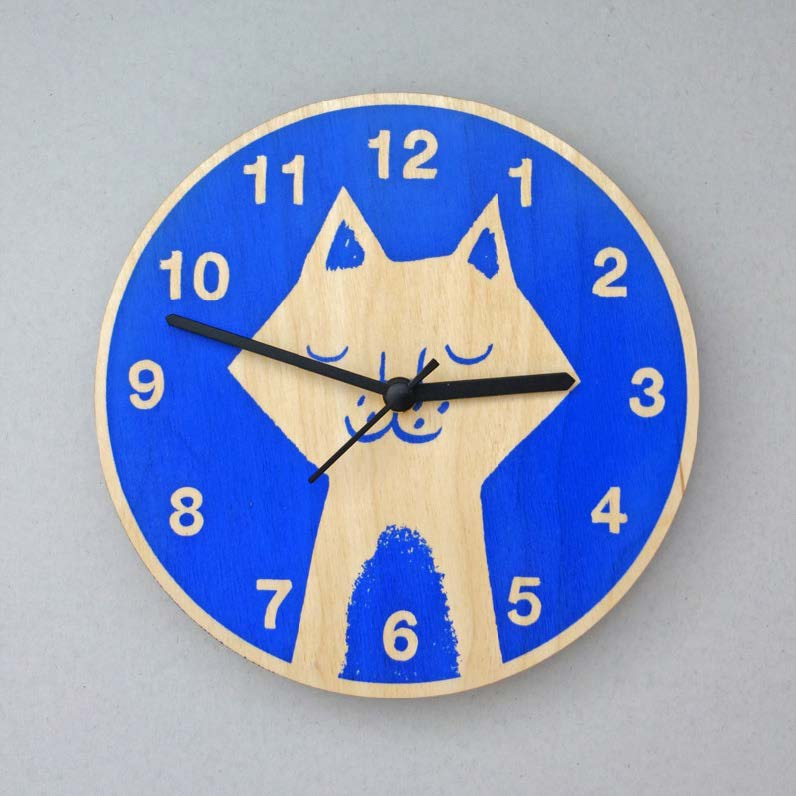
\includegraphics[width=0.5\textwidth]{intro1.jpg}
	\end{frame}

	\begin{frame}
		\frametitle{How to translate hours in minutes?}
		
		\Large
		$x$ - hours
		
		$f(x)=60x$ - conversion in minutes, function
	\end{frame}

	\begin{frame}
		\frametitle{What force is applied to the body?}
		
		\Large
		We know the mass of the body $m$ and its acceleration $a$
		
		What is the force $F$?
	\end{frame}

	\begin{frame}
		\frametitle{What force is applied to the body?}
		
		\Large
		We know the mass of the body $m$ and its acceleration $a$
		
		What is the force $F$?
		
		Newton's second law: $F=ma$
		
		\vspace*{10pt}
		\centering
		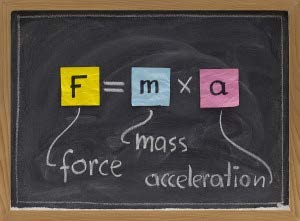
\includegraphics[width=0.4\textwidth]{intro2.jpg}
	\end{frame}

	\begin{frame}
		\frametitle{How to predict the weather?}
		
		
		\centering
		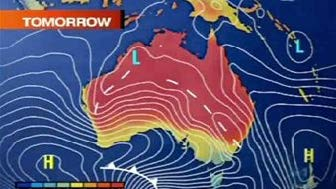
\includegraphics[width=0.6\textwidth]{intro3.jpg}
	\end{frame}

	\begin{frame}
		\frametitle{The Navier-Stokes equations}
		
		
		\centering
		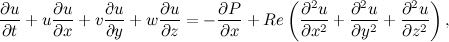
\includegraphics[width=0.8\textwidth]{intro4.jpg}
		
		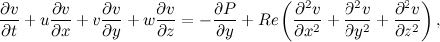
\includegraphics[width=0.8\textwidth]{intro4a.jpg}
		
		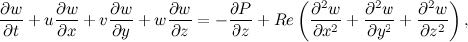
\includegraphics[width=0.8\textwidth]{intro4b.jpg}
		
		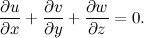
\includegraphics[width=0.25\textwidth]{intro4c.jpg}
	\end{frame}

	\begin{frame}
		\frametitle{The Navier-Stokes equations}
		
		
		\centering
		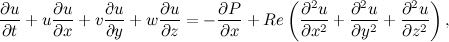
\includegraphics[width=0.8\textwidth]{intro4.jpg}
		
		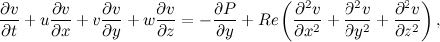
\includegraphics[width=0.8\textwidth]{intro4a.jpg}
		
		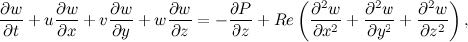
\includegraphics[width=0.8\textwidth]{intro4b.jpg}
		
		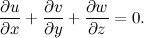
\includegraphics[width=0.25\textwidth]{intro4c.jpg}
		
		\Large
		Differential equations
		
		Allow to find the speed of air and pressure at any point
		
		It's very hard to solve
	\end{frame}

	\begin{frame}
		\frametitle{Sentiment analysis of the text}
		
		\Large
		What is the sentiment of the text?
		
		Options: positive, neutral, negative
		
		Application: automatic analysis of feedback from users
	\end{frame}

	\begin{frame}
		\frametitle{Sentiment analysis of the text}
		
		\Large
		\textit{``Many thanks! Apparently, this is exactly what is not enough for all foreign courses in Machine Learning and Knowledge Discovery. This theory, mathematics, the explanation of what, how it is arranged ``in bowels''.''}
		
		\textbf{What sentiment?}
	\end{frame}

	\begin{frame}
		\frametitle{Sentiment analysis of the text}
		
		\Large
		\textit{``I see a very big minus that the course will be on the ready library sci-kit. The course from Andrew is better that the student himself writes an algorithm and sees from the inside how it works.''}
		
		\textbf{What sentiment?}
	\end{frame}

	\begin{frame}
		\frametitle{Sentiment analysis of the text}
		
		\Large
		$x$ - English text
		
		$f(x)$ - its sentiment (takes values 0, 1, -1)
		
		Can we write out a formula for $x$?
		
		\vspace*{30pt}
		
		At the entrance - not at all numbers
		
		Exact dependence may not exist
	\end{frame}

	\begin{frame}
		\frametitle{More difficult tasks!}
		\Large
		\begin{enumerate}
			\item What will be the demand for the product next month?
			\item How much money will the store earn in a year?
			\item Will the customer return the loan?
			\item Will the patient get cancer?
			\item Will the student pass the next session?
			\item In the photo of the humanities or digithead?
			\item Who will win the battle in the online game?
		\end{enumerate}
		
	\end{frame}

	\begin{frame}
		\frametitle{More difficult tasks!}
		
		\Large
		\begin{enumerate}
			\item Everywhere - very complex implicit dependencies
			\item We can not express them by the formula
			\item But there are a number of examples (texts with a known sentiment)
			\item We will approximate the dependencies using examples
		\end{enumerate}
		
	\end{frame}

	\begin{frame}
		\frametitle{Data analysis and machine learning}
		
		\Large
		It is about how to restore complex dependencies by the finite number of examples
		
		
	\end{frame}

	\begin{frame}
		\frametitle{References}
		
		\Large
		\begin{enumerate}
			\item Gareth James, Daniela Witten, Trevor Hastie and Robert Tibshirani. An	Introduction to Statistical Learning. 2013.
			\item Mohammed J. Zaki, Wagner Meira Jr. Data Mining and Analysis. Fundamental Concepts and Algorithms. Cambridge University Press, 2014.
		\end{enumerate}
		
	\end{frame}

	\begin{frame}
		\frametitle{References}
		
		\Large
		Online courses
		\begin{enumerate}
			\item https://www.coursera.org/learn/machine-learning
			\item https://www.coursera.org/learn/introduction-machine-learning
			\item https://coursera.org/specializations/machine-learning-data-analysis
		\end{enumerate}
		
	\end{frame}

	\section{Basic terms}
	\subsection{2.1}
	\begin{frame}
		\frametitle{Task example}
		\Large		
		\begin{enumerate}
			\item Network of restaurants
			\item We want to open one more
			\item Several siting options
			\item Which of the options will bring the maximum profit?
		\end{enumerate}

		\vspace*{30pt}
		\small
		kaggle.com, TFI Restaurant Revenue Prediction
	\end{frame}

	\begin{frame}
		\frametitle{Notation}
		\Large		
		\begin{enumerate}
			\item $x$ - sample - for which we want to make predictions (the exact location of the restaurant)
			\item $\mathbb X$ - the space of all possible objects (all possible restaurant locations)
			\item $y$ - target - what is predicted (profit during the first year of operation)
			\item $\mathbb Y$ - answer space - all possible values for the answer (all real numbers)
		\end{enumerate}
	\end{frame}

	\begin{frame}
		\frametitle{Training sample}
		\Large		
		\begin{enumerate}
			\item We do not understand anything about the economy
			\item But we have many objects with known answers
			\item $X =(x_i,y_i)^l_{i=1}$ - training sample
			\item $l$ - sample size
		\end{enumerate}
	\end{frame}

	\begin{frame}
		\frametitle{Features}
		
		\Large
		\begin{enumerate}
			\item Objects are abstract entities
			\item Computers only work with numbers
			\item Factors, features - numerical characteristics of objects
			\item $d$ - number of features
			\item $x=(x^1,\dots, x^d)$ - feature description (vector)
		\end{enumerate}
	\end{frame}
	
	\begin{frame}
		\frametitle{}
		
		\Large
		About demography:
		\begin{enumerate}
			\item Average age of residents of the nearest district
			\item Dynamics of number of inhabitants
		\end{enumerate}
	
		About the property:
		\begin{enumerate}
			\item Average cost per square meter of housing nearby
			\item Number of schools, banks, shops, gas stations
			\item Distance to nearest competitor
		\end{enumerate}
	
		About roads:
		\begin{enumerate}
			\item The average number of cars passing by day
		\end{enumerate}
	
	\end{frame}

	\begin{frame}
		\frametitle{Algorithm}
		
		\Large
		\begin{enumerate}
			\item $a(x)$ - an algorithm, a model - function predicting response for any object
			\item Transform $\mathbb X$ into $\mathbb Y$
			\item Linear model: $a(x)=w_1x^1+\dots+w_dx^d$
		\end{enumerate}
	\end{frame}

	\begin{frame}
		\frametitle{Loss function}
		
		\Large
		\begin{enumerate}
			\item Not all algorithms are useful
			\item $a(x)=0$ - will not bring any benefit
			\item The loss function is a measure of the correctness of the algorithm response
			\item Predicted 10,000\$ profit, in fact 5,000\$ -  it is good or bad?
			\item Standard deviation: $(a(x)-y)^2$
		\end{enumerate}
	\end{frame}

	\begin{frame}
		\frametitle{Quality functional}
		
		\Large
		\begin{enumerate}
			\item The quality functional a the quality metric is a measure of the quality of the algorithm work on a sample
			\item Mean Squared Error, MSE: $\frac{1}{l}\sum_{i=1}^l (a(x_i)-y_i)^2$
			\item Less is better
		\end{enumerate}
	\end{frame}

	\begin{frame}
		\frametitle{Quality functional}
		
		\Large
		\begin{enumerate}
			\item Must comply with business requirements
			\item One of the most important components of data analysis
		\end{enumerate}
	\end{frame}

	\begin{frame}
		\frametitle{Learning algorithm}
		
		\Large
		\begin{enumerate}
			\item There is a training sample and a quality functional
			\item The family of algorithms $A$ from what we choose the algorithm (all linear models: $A=\{w_1x^1+\dots+w_dx^d|w_1,\dots,w_d\in \mathbb R\}$)
			\item Training: the search for the optimal algorithm in terms of the functional quality
		\end{enumerate}
	\end{frame}
		
	\begin{frame}
		\frametitle{Machine learning}
		
		\Large
		\begin{enumerate}
			\item Training sample
			\item Feature extraction
			\item Learning model $\rightarrow a(x)$
			\item New object $x \rightarrow $ new prediction
		\end{enumerate}
	\end{frame}

	\begin{frame}
		\frametitle{What you need to know}
		
		\Large
		\begin{itemize}
			\item How to formulate the task?
			\item How to extract the features?
			\item How to form a training sample?
			\item How to choose a quality metric?
			\item How to prepare data for training?
			\item How to train the algorithm?
			\item How to evaluate the quality of the algorithm?
		\end{itemize}
	\end{frame}

	\section{Applications}
	\subsection{3.1}
	\begin{frame}
		\frametitle{Artificial Intelligence}
		
		\centering
		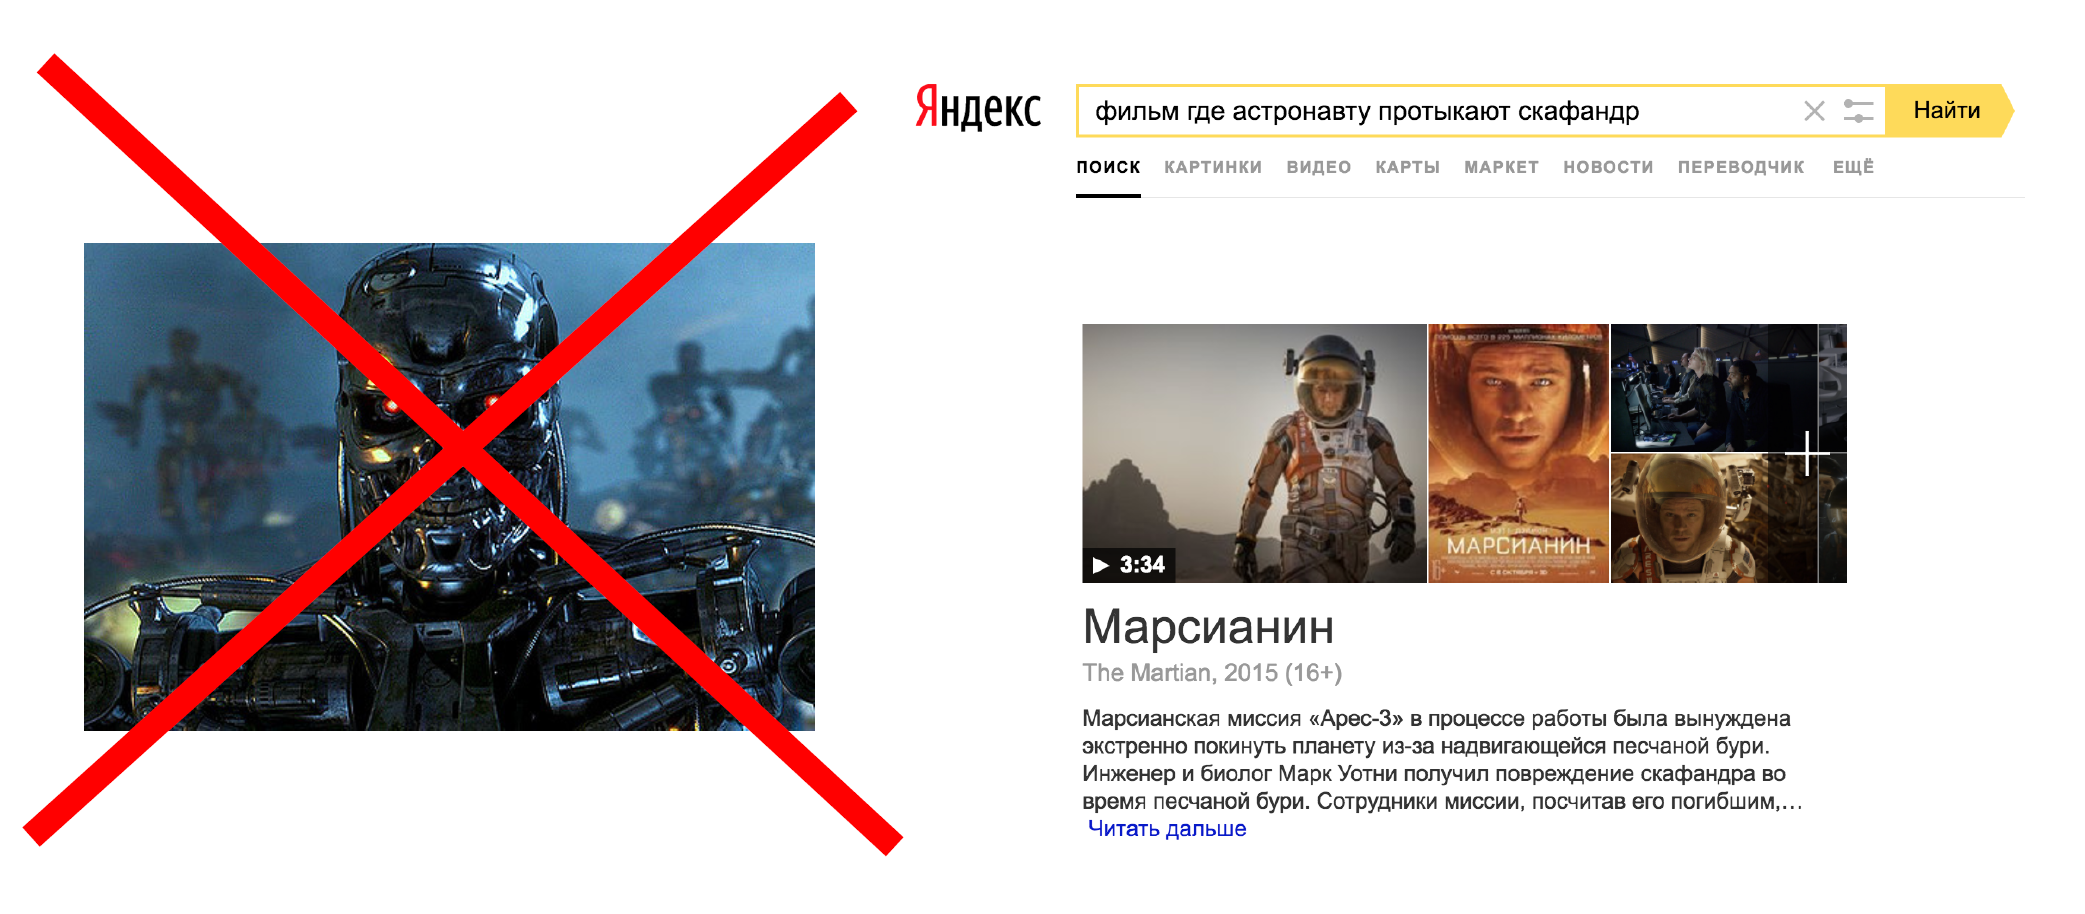
\includegraphics[width=\textwidth]{da_intro1.png}
		\Large
		\begin{enumerate}
			\item Strong AI - in 20-100 years
			\item Specialized AI - now!
		\end{enumerate}
	\end{frame}

	\begin{frame}
		\frametitle{Artificial Intelligence}
		
		\begin{columns}
			\begin{column}{0.5\textwidth}
				\begin{enumerate}
					\item Model for playing Go
					\item Evaluates the success of the turn
					\item Studied by playing with myself
					\item Defeated the world champion in 2017
					\item For a long time, playing in Go was considered an impossible task for a computer
				\end{enumerate}
				
			\end{column}
			\begin{column}{0.5\textwidth}
				\centering
				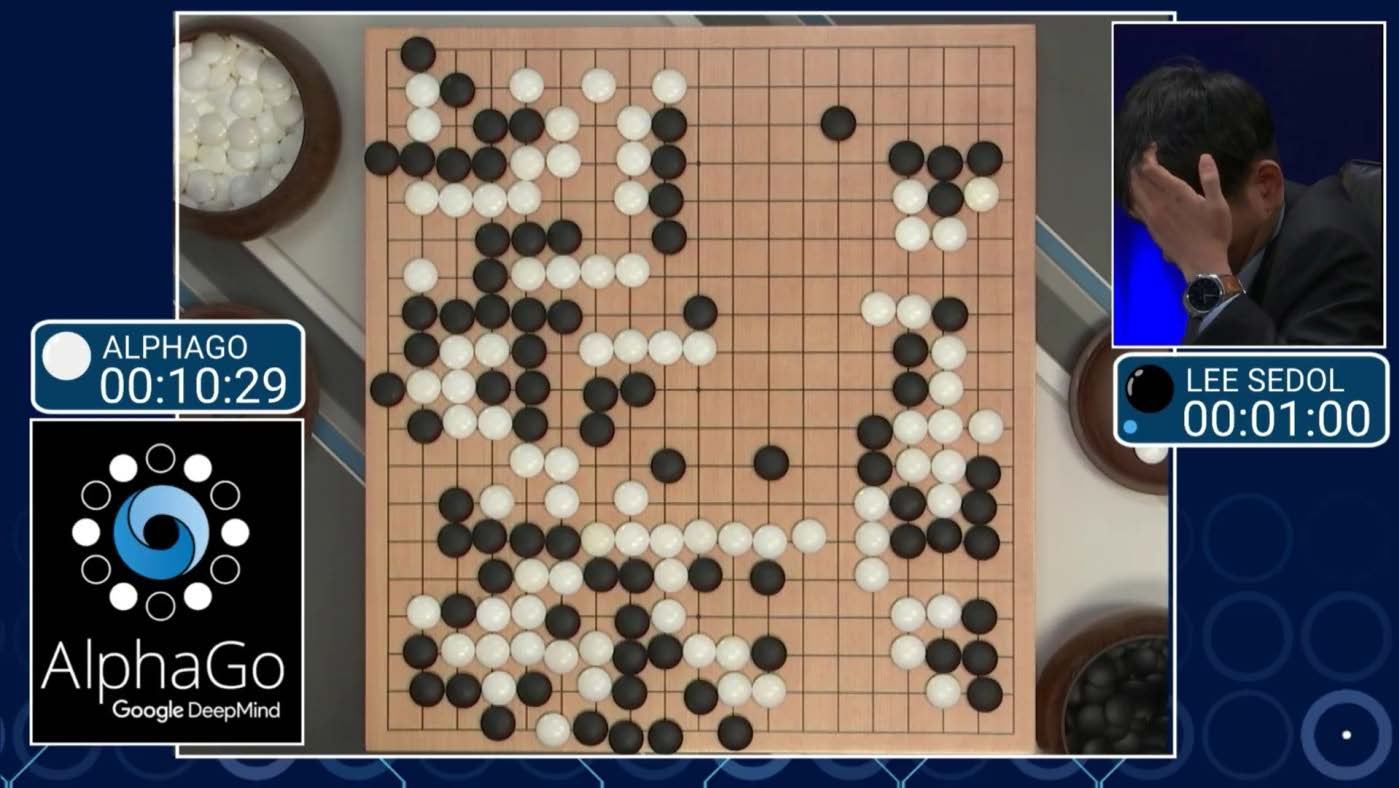
\includegraphics[width=\textwidth]{da_intro2.jpg}
			\end{column}
		\end{columns}

	\end{frame}

	\begin{frame}
		\frametitle{Annotating images}
		
		\centering
		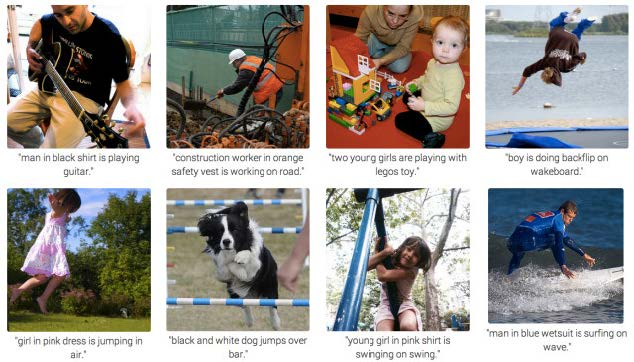
\includegraphics[width=\textwidth]{da_intro3.jpg}
	\end{frame}

	\begin{frame}
		\frametitle{Style transfer}
		
		\centering
		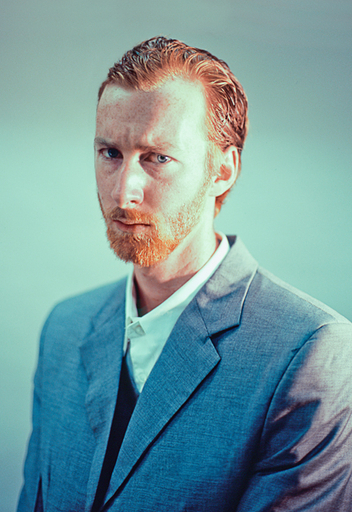
\includegraphics[width=0.4\textwidth]{da_intro4.jpg}\hspace*{10pt}
		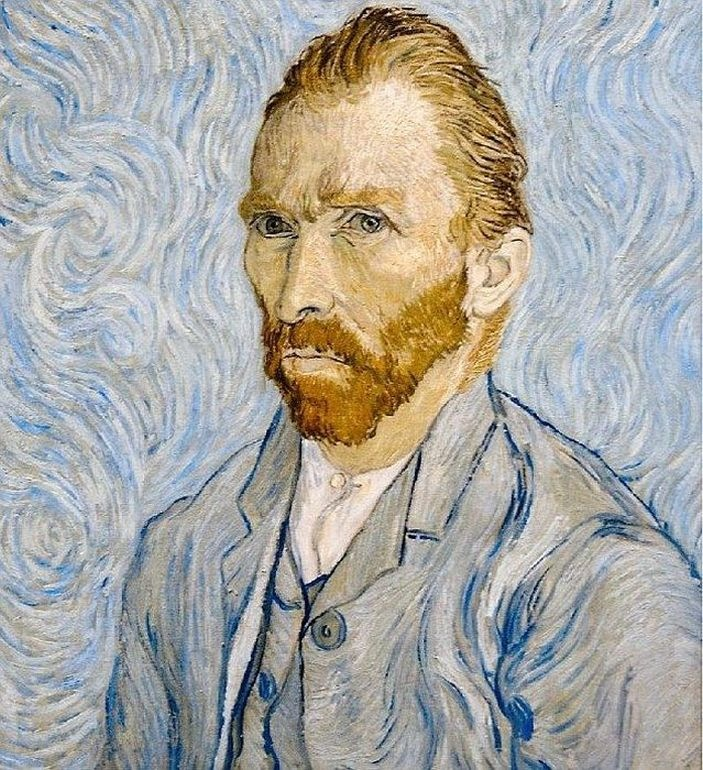
\includegraphics[width=0.53\textwidth]{da_intro5.jpg}
	\end{frame}

	\begin{frame}
		\frametitle{Artificial Intelligence}
		
		\begin{columns}
			\begin{column}{0.5\textwidth}
				\begin{enumerate}
					\item The model predicts whether the required chemical composition is obtained in 		result of melting
					\item Reduces the consumption of ferroalloys by 5\%
					\item Savings of up to 23 million rubles per month
					\item Joint project of Yandex and Magnitogorsk metallurgical Combine
				\end{enumerate}
				
			\end{column}
			\begin{column}{0.5\textwidth}
				\centering
				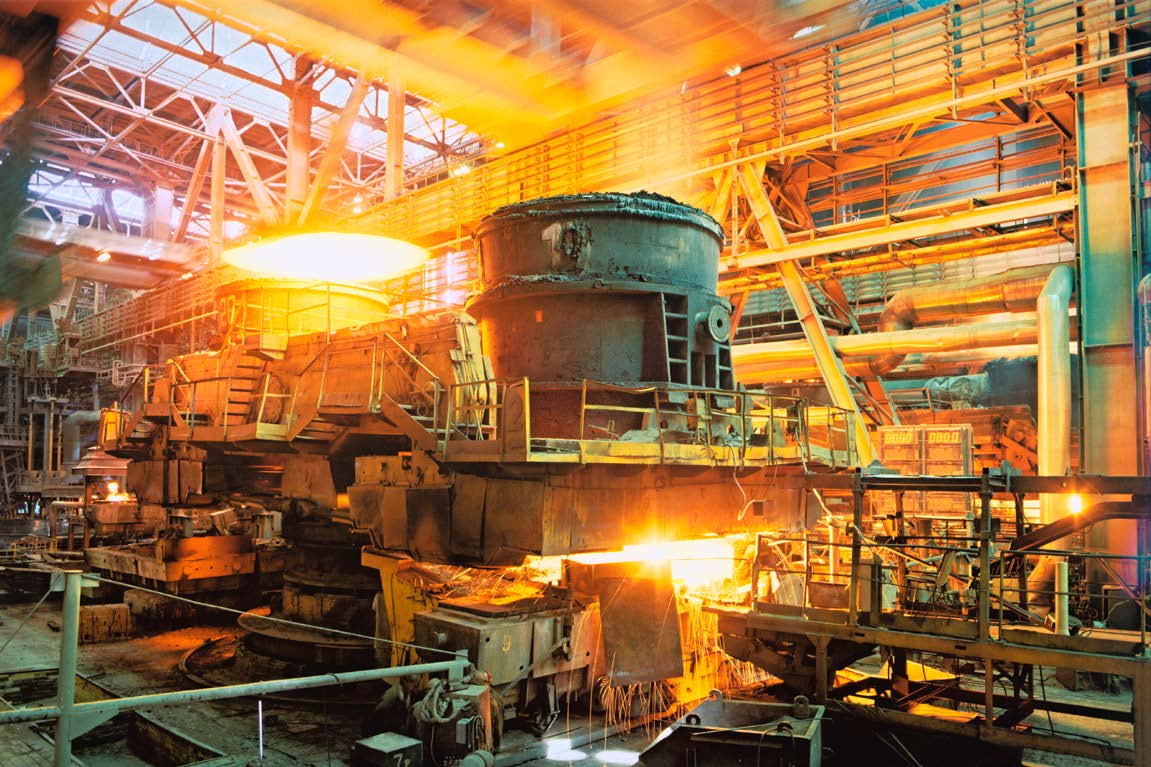
\includegraphics[width=\textwidth]{da_intro6.jpg}
			\end{column}
		\end{columns}

	\end{frame}

	\begin{frame}
		\frametitle{Recommender systems}
		
		\centering
		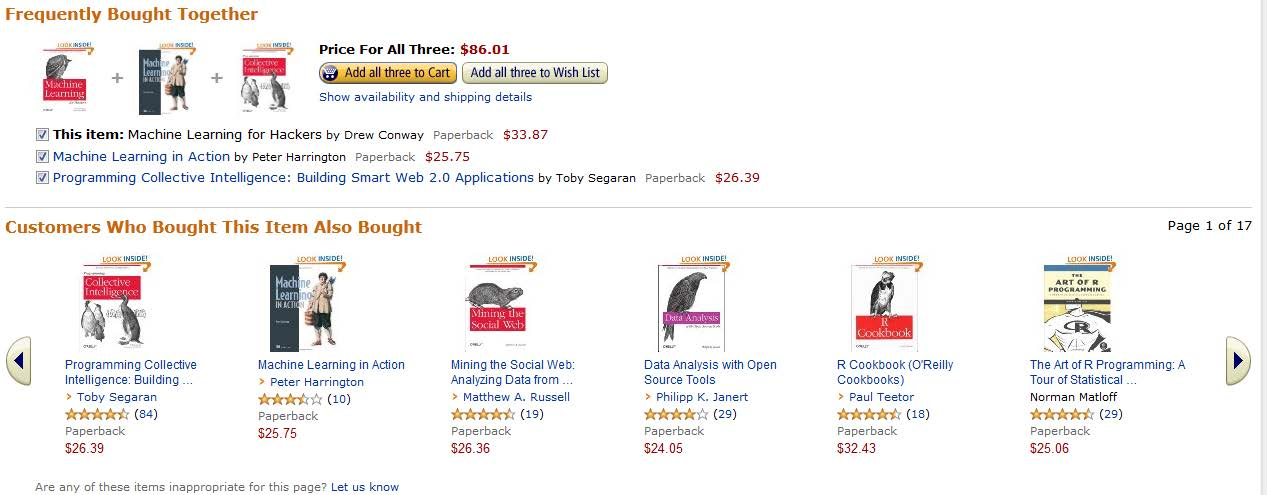
\includegraphics[width=\textwidth]{da_intro7.jpg}

		\begin{itemize}
			\item Shelves of recommendations on Amazon generate 35\% of all purchases
			\item Recommendations based on machine learning and analysis of large volumes of data
		\end{itemize}
	\end{frame}

	\begin{frame}
		\frametitle{Why is this necessary?}
		
		\Large
		\begin{itemize}
			\item That's cool
			\begin{itemize}
				\item Challenges
				\item Movement towards artificial intelligence
			\end{itemize}
			\item This is useful
			\begin{itemize}
				\item Profit from data
				\item Data-driven companies
				
			\end{itemize}
		\end{itemize}

	\end{frame}

	\begin{frame}
		\frametitle{How can you analyze data?}
		
		\Large
		\begin{itemize}
			\item Data scientist
			\begin{itemize}
				\item Working with data
				\item Knowledge of tools and methods
				\item Experience in solving problems
			\end{itemize}
			\item Manager
			\begin{itemize}
				\item Understanding how machine learning works
				\item Understanding bottlenecks, estimating deadlines
			\end{itemize}
			\item Customer
			\begin{itemize}
				\item Quality metrics
				\item Data requirements
				\item Limitations of modern approaches
			\end{itemize}
		
		\end{itemize}
		
	\end{frame}
\end{document}
	
	
